\setcounter{chapter}{0}
\chapter{Introduction}
\section{Problématique et besoins}
\paragraph{}
Durant la partie I, nous avons du concevoir nous même un moteur d'inférence utilisant le lange JAVA, cependant il serait plus intéressant de remplacer ce moteur basique par une moteur plus performant et plus adéquat aux système multi-agent, ce qui nous a amené a l'utilisation de la plateforme JASON.
\section{Définitions}
\subsection{Architecture CDI (Croyance-Désir-Intention)}
\paragraph{}
Une architecture BDI est conçue en partant du modèle "Croyance-Désir-Intention", en anglais "\textbf{Belief-Desire-Intention}", de la rationalité d'un agent intelligent. tel que les \textbf{croyances} sont les informations que l'agent possède sur l'environnement et sur d'autres agents qui existent dans le même environnement, les \textbf{désirs} représentent les états de l'environnement, et parfois de lui-même, que l'agent aimerait voir réalisés et finalement les \textbf{intentions} d'un agent sont les désirs que l'agent a décidé d'accomplir ou les actions qu'il a décidé de faire pour accomplir ses désirs( Même si tous les désirs d'un agent sont consistants, l'agent peut ne pas être capable d'accomplir tous ses désirs à la fois)
\subsection{AgentSpeakL}
\paragraph{}
AgentSpeak est un langage orienté agent. il est basé sur la programmation logique(Prolog) et les architectures CDI pour les agents cognitives.
\begin{figure}[H]
	\centering
	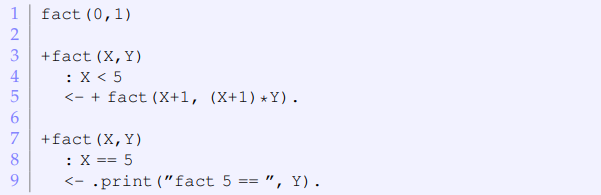
\includegraphics[width=\textwidth]{imgs/agenttSpeak.png}
	\caption{Exemple d'un agent voulant calculer le factoriel d'un nombre}
\end{figure}
\subsection{La plateforme JASON}
JASON est une plateforme qui a pour but de faciliter le développement de système multi-agent en offrant un environnement de travail complet comportant un éditeur de texte, un débogger et un compilateur AgentSpeak.